\section{Introduction}
In Belgium one man in three and one woman in four face cancer before their 75th
birthday \cite{kanker} In 2010, 62.017 new cases of cancer were diagnosed
accroding to \cite{kankerliga}. Moreover, the World Health Organisation
estimates the worldwide death toll from lung cancer will be 10.000.000 by 2030,
which makes it one of the deadliest cancers \cite{gu, zheng}. But an early
detection can increase the survival rate up to 70-80\% \cite{swensen} and
broadens the amount of treatment options \cite{greenlee}. Therefore, a wide
range of studies have focussed on this topic. The only way to detect lung cancer
in an early stage is by examining a patient's scan carefully. However, even for
an experienced radiologist detecting all nodules on a scans is not trivial and
there is an increasing demand for methods that provide assistance for this
difficult task.

Currently, expert radiologists perform the investigation of the computed
tomography (CT) scans. They use the shape, the texture, the location and the
growth rate of the volume of the nodule as clinical parameters to determine the
malignancy of the nodules and to decide on the diagnosis of lung cancer. A
jagged shape nodule is more likely to be lung cancer than a smooth one. A fatty,
bony, watery nodule or a mixture of these different contents is less likely to
indicate lung cancer than a nodule that is attached to a vessel. A nodule
attached to the lung wall is typically diagnosed as benign if the
volume-doubling periode is longer than 400 days \cite{wu}. Nevertheless, the
examination of these scans is a time-consuming task and is not free from errors.
Fortunately, due to recent developments in CT technology it is possible nowadays
to obtain near isotropic, submillimeter resolution images of the complete chest
in a single breath hold. This high resolution has the advantage that it enables
visualisation of small and low-contrast nodules that could hardly be screened in
conventional programs. But although small nodules are in principle detectable in
CT scans, a non-negligible fraction may be overlooked if they are situated in a
maze of vessels of similar size \cite{ozekes}. An example of a nodule hidden in
a maze of vessels is shown in \autoref{nodmaze}.
\begin{figure}[htp]
\begin{center}
  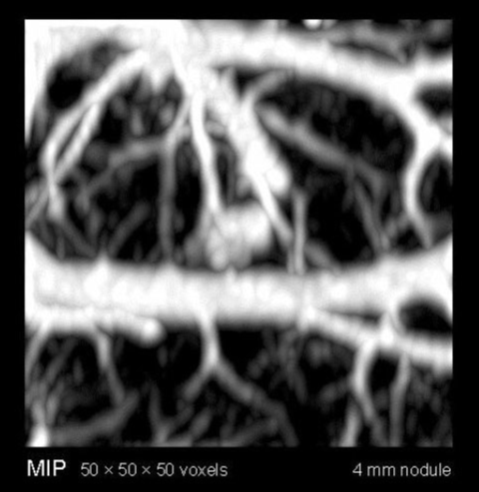
\includegraphics[width= 30 mm]{img/noduleMaze.png}
  \caption{Nodule in maze of vessels of similar size \cite{wiemkerfig}.}
  \label{nodmaze}
\end{center}
\end{figure}
The downside of these recent developtments towards high resolution images is
that enormous amounts of data are generated which increase the work load of radiologists.
Especially since low-dose CT scans are more and more implemented in routine
screenings. Still, this is no idle measure. Long nodules are very commonly
detected on CT scans. Research shows that up to 51\% of smokers aged 50 years or
older have pulmonary lung nodules on CT scans \cite{mahon}. Therefore, the
United States Preventive Services Task Force stated that it ``recommends annual
screening for lung cancer with low-dose computed tomography (LDCT) in adults
aged 55 to 80 years who have a 30 pack-year smoking history and currently smoke
or have quit within the past 15 years'' \cite{ups}. This workload might lead to
a higher amount of undetected nodules per scan as the radiologist has
less time to spend per patient and long working hours and fatique become
unavoidable. This trend will contribute to an increased intra- and
interreader variability amongst radiologists \cite{armato, hens}. No wonder the
detection of pulmonary nodules from volumetric CT scans is one of the most studied computer-aided detection (CAD) applications
\cite{sluimer}. There is a need for a CAD system that can assist the radiologist
in the detection of pulmonary nodules.

The goal of this project is to develop a fully automated algorithm for the
detection of pulmonary nodules in CT scans. The algorithm will be established as
a cascaded classifier which is a robust and fast machine learning algorithm.
This algorithm will classify each voxel of the 3D images an assign a
nodule-probability to each voxel. One of the challenges is the selection of the
features that will be extracted from the image. The fact that some nodules are
embedded in surrounding tissue (e.g.
lung wall, blood vessel, etc.) and the fact that some nodules demonstrate very
irregular shapes prevents us from using simple spherical template matching which
might seem an obvious choice at first for pulmonary lung detection. In order to
select the right classifier and list of features a non-exhaustive literature
review is performed. Commercial and non-commercial CAD systems for nodule
detection and their performances are discussed. Of course, in order to design an
accurate and efficient CAD system, one needs to understand the biology of lung
nodules so that topic is also briefly touched.

Then a short theoretical background on image processing, with a focus on feature
extraction and selection, and machine learning are provided. Both topics
are related to findings in the literature. The statistical measures used for
assessing the performance of classifiers, and algoirthms or statistics in
general, are also briefly discussed as they might not be trivial in this
project.

The methodology that was established in this project is explained from the
acquisition of the datasets and the preprocessing of the data till the training,
testing and validating of the algorithm. The advantages and disadvantages of
every step are discussed and the final results are presented. Finally, the main
conclusions from the projected were summarized and suggestions for future
research are made.

In the appendix the reader can find the reports of the weekly meetings with the
supervisors, the Ganttchart and the timeschedule which present together the
logbook of the project.








